\chapter{Active Directory Tier 0 Security Framework: Cyberattack Prevention and Protection Against Advanced Threats}

\abstract{The Active Directory (AD) Tier 0 Security Framework is a critical component in the defense-in-depth strategy of any enterprise network. Tier 0 assets—Domain Controllers (DCs), domain-joined privileged accounts, and the AD schema itself—represent the crown jewels of an organization’s identity infrastructure. Their compromise leads to complete domain dominance and long-term persistence by adversaries.
This work presents a comprehensive approach that defender's can use to securing Tier 0 by integrating hardening best practices, identity segmentation, Privileged Access Management (PAM), and continuous monitoring. Emphasis is placed on mitigating lateral movement, credential theft, and Advanced Persistent Threats (APTs) through the application of the Principle of Least Privilege (PoLP), Just-in-Time (JIT) access, and secure administrative workflows.
Additionally, the framework addresses attacker techniques such as Pass-the-Hash (PtH), Golden Ticket, DCShadow, and DCSync, mapping each to specific mitigation, detection, protection, and prevention strategies. By implementing the Tier 0 Security Framework, defenders can significantly reduce an organization's attack surface and increase its resilience against both commodity malware and nation-state actors targeting their Active Directory (AD) infrastructure.}

\section{Introduction to Active Directory Tier 0: Rebuilding Trust and Post-Breach Remediation}
This chapter outlines a strategic and technical framework for executing remediation operations in the aftermath of a significant cybersecurity incident affecting Active Directory (AD) infrastructure. Specifically, it focuses on the processes required to regain control over a compromised identity and directory infrastructure and restore secure, functional operations across Tier 0 assets.

Remediation refers to the act of reclaiming authority over a compromised environment and reconstructing its core trust components. This includes, but is not limited to, Domain Controllers, privileged identities, and related infrastructure dependencies that constitute the backbone of \textit{Identity and Access Management (IAM)}.

The guidance provided within serves as part of the broader technical methodology that supports AD remediation and hardening. It offers a foundational reference for defenders and security teams charged with orchestrating recovery operations-particularly those tasked with rebuilding the trusted core of Active Directory in a post-breach environment.

{\emergencystretch=3em
%Structured around the \textit{Containment\-/Eviction\-/Eradication\-/Rebuild} (CEER) model, ...
}

This content is designed for defenders, white hat hackers, and blue team operators, incident response engineers, and Active Directory administrators responsible for technical execution during crisis recovery operations. While strategic in nature, its primary focus is operational-providing actionable and meaningful direction for secure reconstruction in high-risk Active Directory environments.

\section{Strategic Scenarios for Active Directory Tier 0 Remediation}
Before diving into specific remediation scenarios, it is first important to contextualize the role of Tier 0 in the broader Active Directory security architecture. Tier 0 assets-Domain Controllers, Domain Admin accounts, and other privileged information systems-represent the most critical components of any identity infrastructure. As such, their compromise can result in full domain takeover. The following scenarios are designed to address common security gaps, misconfigurations, and legacy design flaws, each providing the reader with a practical blueprint for understanding how to proactively and aggressively defend and reclaim control over Tier 0 resources. Whether you are implementing these strategies proactively or as part of an incident response effort, they offer actionable steps rooted in real-world defensive security practices.

\section{Objectives and Operational Context}
This chapter establishes a practical framework for conducting Tier 0 remediation operations following a security breach, aligning with three distinct strategic scenarios that guide the broader recovery processes.

\subsection{Scenario 1: Rapid Restoration of Mission-Critical Services}
\begin{itemize}
    \item Prioritizes immediate business continuity by restoring mission-critical and business imperative systems while managing residual risk.
    \item Assumes that Tier 0 assets may be partially compromised but focuses more on restoring service availability with controlled exposure.
    \item Utilizes containment and eradication strategies and compensating controls to enable safe operations while full remediation efforts proceed in parallel.
\end{itemize}

\subsection{Scenario 2: Regaining Full Control Over the Information System (IS)}
\begin{itemize}
    \item Focuses on neutralizing the attacker's toehold and reasserting authoritative control over Active Directory (AD) and related Tier 0 assets.
    \item Involves the re-establishment of broken trust boundaries, reconfiguring privileged access pathways, and verifying and validating the integrity of critical authentication infrastructures.
\end{itemize}

\subsection{Scenario 3: Building a Long-Term Foundation for Secure IT Operations}
\begin{itemize}
    \item Leverages the incident response effort to re-architect trust boundaries and implement lasting improvements to enterprise security.
    \item Emphasizes strategic planning, including the redesign of privileged access models, implementation of tiered administration levels, and the hardening of identity infrastructure information systems and assets.
    \item Shifts focus from tactical recovery to sustainable security posture management via security policy enforcements, continuous monitoring efforts, and operational cybersecurity maturity.
\end{itemize}

Depending on the scenario selected, specific remediation goals must be defined-particularly for the \textbf{safe eviction of adversaries} and the \textbf{re-establishment of Tier 0 trust boundaries.} The technical measures presented throughout this chapter are designed to meet those objectives.

This content supports defenders in aligning remediation activities with both short-terms business needs and long-term cybersecurity maturity. By anchoring technical efforts to clearly defined strategic outcomes, defenders will find themselves establishing and achieving both effective recovery and lasting resilience.

\section{Scope and Limitations}
This chapter is not intended to serve as a rigid, step-by-step remediation playbook. Each security incident presents unique variables-ranging from the attacker's \textit{Tactics, Techniques, and Procedures (TTPs)} to the organization's business priorities and operational constraints. Effective remediation requires contextual adaptation of the principles outlined herein.

While this chapter presents a comprehensive technical foundation for regaining control over compromised Tier 0 assets, it is imperative that defenders and organizations tailor their remediation road-map based on specific, situational intelligence applicable to the organizations risk landscape and network security posture requirements. The technical guidance should be preferably be interpreted through collaboration with Active Directory subject matter experts-whether internal, vendor-based, or third-party service providers.

Remedial efforts should never solely rely on ad hoc decisions, improvised foxes, or from the flawed notion of \textit{security through obscurity}-even when under pressure. Such missteps can worsen the situation at hand, further compromise information system integrity, and jeopardize long-term security objectives.

Finally, while this chapter focuses on addressing some of the most common attack vectors leveraged by adversaries in Active Directory environments, additional actions may be required to neutralize threats specific to the incident at hand. Defenders and security teams must remain adaptive and vigilant, supplementing the prescribed technical actions as needed to fully and safely evict the threat actor and restore control of the environment.

\section{Key Concepts: Tiered Administration Model}
A foundational principle in Active Directory (AD) security architecture is the \textbf{tiered administration model}, designed to mitigate unauthorized privilege escalation and reduce the blast radius of a compromised account or information system. Originally formalized by Microsoft, this model segments administrative control into three distinct tiers, each with a defined security boundary and role in the enterprise ecosystem.

\subsection{Tier 0-Red Tier: The Trusted Core}
Tier 0 encompasses the most critical assets within the identity infrastructure-resources that directly control authentication, authorization, and domain-wide security posture. This includes:

\begin{itemize}
    \item Domain Controllers (DCs)
    \item AD schema and configuration partitions
    \item Privileged security groups (e.g., Domain Admins (DAs), Enterprise Admins (EAs)
    \item \textit{Active Directory Federation Services (AD FS)
    \item Active Directory Domain Services (AD DS)}
    \item Tier 0 management systems and consoles
\end{itemize}

Because Tier 0 governs the entire identity and access control plane, it must be isolated from all other tiers. These assets are considered mission-critical because a compromise at this level enables total domain control. Access to Tier 0 should be highly restricted, isolated, and managed with the most rigorous security controls. In addition, only highly trusted authorized and certified personnel with a need to know and applicable business justification should interact with Tier 0 systems. A detailed methodology for identifying and scoping Tier 0 assets is provided in the appendix.

\subsection{Tier 1-Yellow Tier: Business-Critical Systems}
Tier 1 consists of systems that enforce or execute business logic-servers, applications, and services essential to organizational operations and workflows. While these information systems are vital, they do not directly control identity infrastructure. Examples include:
\begin{itemize}
    \item Line-of-Business (LOB) applications
    \item SQL and Application servers
    \item Middleware platforms
    \item \textit{Enterprise Resource Planning (ERP)} systems
\end{itemize}

Administrative accounts and tools for Tier 1 must never have access to Tier 0 resources, and vice versa.

\subsection{Tier 2-Green Tier: End-User Devices and Peripherals}
Tier 2 comprises user-facing endpoints and peripheral systems. These include:
\begin{itemize}
    \item User workstations and laptops
    \item Printers and scanners
    \item \textit{Mobile Device Management (MDM)} platforms
    \item \textit{Internet of Things (IoT)} or non-critical infrastructure
\end{itemize}

Tier 2 environments are typically the most exposed segment of an enterprise network, encompassing user workstations, laptops, and other general-purpose endpoints. Because they interface directly with email, web browsers, removable media, and cloud-based applications, they present the broadest attack surface and thus introduce common entry points and attack vectors for attackers to penetrate. As such, Tier 2 administrators and defenders must be strictly separated from Tier 1 and Tier 0 domains to prevent lateral movement.

From both a defensive and offensive standpoint, a compromise at this tier carries significant implications.

\section{An Defender's View on What a Tier 0 Compromise Means}
From a defender's viewpoint, Tier 0 is the front line of an organization's complete security posture. A successful breach of a Tier 2 asset can be just as devastating compared to a Tier 0 breach and can have cascading effects of epic proportions if not properly contained.

Entry points and attack vectors a defender needs to be aware of when dealing with Tier 2 assets is listed below.

\begin{itemize}
    \item \textbf{Entry Point for Malware and Phishing Campaigns:} Endpoints in Tier 2 are often the target of spearphishing, drive-by downloads, and malicious email and file attachments. A compromised user endpoint device can become a beachhead for malware deployment or ransomware execution.
    \item \textbf{Credential Exposure Risks:} Tier 2 machines frequently cache user credentials or are used to perform routine administrative tasks, especially in poorly segmented environments. If privileged credentials are ever exposed or reused on these information systems, attackers may harvest them using tools like \textbf{Mimikatz} or \textit{LSASS (Local Security Authority Subsystem Service)} dumps.
    \item \textbf{Lateral Movement Vectors:} If strict administrative separation is not enforced, a compromised Tier 2 endpoint can be used to pivot into Tier 1 (server infrastructure) or even Tier 0 (identity infrastructure). For example, if help desk or junior admins with broader access log into Tier 2 systems, their elevated tokens become valuable targets.
    \item \textbf{Impact on Incident Response (IR):} A breach in Tier 2 may require wide-scale endpoint investigations, imaging, or re-imaging-consuming IR and S\textit{OC (Security Operations Center)} resources. Without proper network segmentation, one compromised device can lead to rapid spread through endpoint-to-endpoint movement.
    \item \textbf{Loss of User Trust and Operational Disruption:} Widespread Tier 2 compromise often results in downtime for employees, disruptions to critical business operations, and a loss of confidence by the end-user and stakeholders in ITs (Information Technology) ability to safeguard information systems.
\end{itemize}
    
This hierarchical model is central to implementing secure administrative security boundaries. It underpins many of the technical actions described in later sections of this chapter, particularly around account separation, access control, and trust rebuilding in post-breach scenarios.

\section{An Attacker's View on What a Tier 0 Compromise Means}
From an attacker's view, Tier 2 is the low-hanging fruit-the ideal springboard for deeper infiltration into the internal network.

\begin{itemize}
    \item \textbf{Initial Toehold and Persistence:} Tier 2 information systems are typically where attackers first gain access-through phishing, social engineering, browser exploits, or infected USB drives; however, once inside, adversaries often deploy \textit{Remote Access Trojans (RATs)}, and begin either passive or active reconnaissance activities.
    \item \textbf{Credential Harvesting and Escalation:} Attackers are known to dump credentials or hash values from Tier 2 machines to identify any higher-privileged users. If local administrator accounts share passwords across machines, \textit{Pass-the-Hash (PtH)} or \textit{Local Privilege Escalation (LPE)} can quickly lead to broader access and more devastating compromise.
    \item \textbf{Network Reconnaissance and Target Selection:} Compromised Tier 2 information systems allow attackers to map the targeted environment using tools like \textbf{BloodHound}, \textbf{SharpHound}, or \textbf{PowerView}. This reconnaissance helps to identify domain trusts, service accounts, and high-valued targets.
    \item \textbf{Lateral Movement:} By exploiting misconfigurations, for example, \textit{Unconstrained Delegation}, admin sessions, or \textit{SMB (Server Message Block)} shares, attackers can pivot to Tier 1 information systems, eventually aiming for Tier 0. A single overlooked Tier 2 workstation can become the key to domain ownership.
    \item \textbf{\textit{Living-Off-The-Land (LoTL)} Techniques}: Modern attackers often avoid dropping binaries. Instead, they abuse native Windows tools such as PowerShell, Sysinternals PsExec, and Certutil (to name a few) on Tier 2 machines to remain stealthy, bypass security detection measures, and blend effortlessly into legitimate user behaviors.

In sum, a Tier 2 compromise might seem minor on the surface-after all, it is "just a user machine." But in reality, it is often the first domino to fall in a full-domain breach. From a defensive standpoint, this makes Tier 2 hygiene, segmentation and monitoring absolutely essential. From an offensive perspective, Tier 2 is a fertile playground for exploitation, especially in organizations that have not implemented strict tier separation or credentialed boundaries.

Hardening Tier 2 is not just a best practice-it is a necessary critical security control in preventing the escalation chain that ultimately leads to Tier 0 compromise.

\subsection{Understanding the Trusted Core}
In the context of enterprise cybersecurity and \textit{Incident Response (IR)}, the term \textbf{trusted core} refers to the most sensitive components of the information system-those whose compromise would signify systemic risk across the entire infrastructure. The trusted core contains the \textbf{most critical components of the identity infrastructure}-the systems and entities that \textbf{must remain uncompromised} for the entire security model to remain intact.

The trusted core encompasses services and information systems that are foundational to control, governance, and security. If an attacker gains control over any element within this core, defenders must assume that the \textbf{entire environment is compromised.}

\subsection{Trusted Core Components}
The trusted core encompasses the most critical information systems and services that uphold the security and integrity of the enterprise identity infrastructure. While not exhaustive, it typically includes the following components:

\subsection{Identity and Access Management (IAM)}
Core identity services such as Active Directory Domain Services (AD DS), underlying authentication databases, and Kerberos ticketing infrastructure responsible for verifying and issuing identity claims across the environment.

\subsection{Virtualization Management Platforms}
Hypervisor hosts and their management consoles, including information systems such as VMware or Microsoft Hyper-V Manager. These platforms often host Tier 0 assets and must be protected to prevent indirect control over the domain.

\subsection{Privileged Administrative Infrastructure}
Information systems used to administer high-privileged environments, including \textit{bastion hosts}, \textit{jump servers}, dedicated administrative consoles, and \textit{Privileged Access Management (PAM)} solutions. These components facilitate access to Tier 0 information systems and are a prime target for attackers seeking elevation.

\subsection{Security Monitoring and Detection Systems}
Centralized platforms that oversee detection, logging, and incident response-such as \textit{Security Information and Event Management (SIEM)} systems, \textit{Endpoint Detection and Response (EDR)} tools, and audit logging infrastructures. Compromising these components blinds defenders and allows attackers to operate with sheer impunity.
\end{itemize}

In secure Active Directory enterprise architectures \textbf{minimizing the scope and complexity of the trusted core} is a key design goal. A smaller, well-defined core is easier to harden, monitor, and rebuild in the event of a breach. Overextension introduces unnecessary exposure and increases the likelihood of human-error and misconfigurations.

\subsection{Trusted Core in Active Directory Environments}
Within an Active Directory (AD) deployment, the trusted core is tightly aligned with the \textbf{Tier 0 assets}, as defined in the previous section. This includes the entire authentication infrastructure and any information system that can exert control over it. Accordingly, any compromise at this level requires immediate containment and a comprehensive rebuild of trust.

\subsection{Security Implications}
Because of its systemic importance, the trusted core must be:

\begin{itemize}
    \item \textbf{Logically and physically isolated} from lower-tiered environments (Tiers 1 and 2).
    \item \textbf{Administered using hardened, purpose-built accounts and devices.}
    \item \textbf{Monitored continuously for signs of unauthorized access or anomalous behaviors.}
\end{itemize}

By maintaining a lean and clearly scoped trusted core, defenders can improve incident response agility, reduce lateral movement opportunities, and re-establish control faster during a crisis.

\subsection{Privileged Groups in Active Directory}
In an Active Directory (AD) environment, \textbf{privileged groups} are built-in security groups that hold extensive administrative rights over the domain, forest, or specific informational subsystems within the core directory infrastructure. These groups can directly manage or elevate privileges within the environment and are, therefore, high-valued targets for adversaries seeking domain dominance.

Compromise of any privileged group can grant an attacker complete control over Tier 0 assets and, by extension, the entire identity infrastructure. These groups must be tightly monitored, strictly controlled, regularly audited, and properly isolated from lower-tiered administrative scopes.

\section{Critical Privileged Groups}
Below is a list of key native privileged groups and their associated risks:

\subsection{Administrators}
Full control over the domain; members can modify any setting or object in Active Directory.

\subsection{Domain Controllers (DCs)}
Represents all domain controllers, including
\textit{Read-Only Domain Controllers (RODCs)}
and
\textit{Backup Domain Controllers (BDCs).}
Any compromise here directly will impact the authentication infrastructure.

\subsection{Schema Administrators}
Can modify the AD schema, allowing changes to the directory structure and behavior-potentially enabling stealthy persistence mechanisms.

\subsection{Enterprise Administrators (EAs)}
Forest-wide privileges across all domains; this group is rarely needed in daily operations and should remain empty whenever possible.

\subsection{\textbf{Domain Administrators (DAs)}}
Grants full administrative access within the domain, including the ability to read sensitive data from the secrets database (for example, \textit{New Technology LAN Manager (NTLM)} hashes and Kerberos tickets). These accounts are capable of extracting credentials for all privileged users.

\subsection{Key Administrators / Enterprise Key Administrators}
Manages keys and certificate attributes used in Windows Hello for Business. They can assign cryptographic credentials, and in environments with certificate-based authentication, impersonate privileged users by generating and assigning certificates-even for domain controllers-unless protected by \texttt{adminSDHolder.}

\subsection{Account Operators}
Can create, modify, and delete most user, computer, and group accounts-except those protected by \texttt{adminSDHolder.} Improper use or compromise of this group enables mass user manipulation.

\subsection{Server Operators}
Have the ability to log on locally and manage servers, including domain controllers. Their privileges can be used to access or dump sensitive credentialed material.

\subsection{Backup Operators}
Can back up and restore files, including the Active Directory database (\texttt{NTDS.dit}) from a domain controller-making it possible to extract and crack all stored secrets offline.

\subsection{Print Operators}
Can install printer drivers on domain controllers. A common abuse path involves loading a \textbf{malicious driver} to execute code in kernel mode, thereby gaining \texttt{SYSTEM}-level access and extracting credentials.

\section{Security Implications}
Because of their ability to manipulate domain-wide configurations and operations, extract secrets, and escalate privileges, these groups are frequently targeted by adversaries after initial access and toehold has been established. Common tactics include:
\begin{itemize}
    \item \textbf{Privilege escalation through token theft or \textit{SID (Security Identifier)} abuse}
    \item \textbf{Persistence via rogue additions to privileged groups}
    \item \textbf{Credential theft using tools like Mimikatz or DCSync}
\end{itemize}

    Additionally, \textbf{mitigation measures} include:
    \begin{itemize}
        \item Minimizing group membership and maintaining strict access controls
        \item Implementing monitoring and alerting for group membership changes
        \item Enforcing tier isolation and Just-In-Time (JIT) administrative access
        \item Applying protections such as \texttt{adminSDHolder} and Credential Guard mechanisms
    \end{itemize}

Effective defense starts with a clear inventory of privileged groups and a deep understanding of their security impacts and implications. In an incident recovery scenario, validation and cleansing of these groups is a critical task during the rebuild of Tier 0 trust.

\section{Understanding the Criticality of Control Paths in Active Directory}
A \textit{control path} is a logical chain of control relationships between security principals (users, groups, computers) in an Active Directory (AD) environment. Each link in the path represents a privilege or property that allows only one entity to exert influence or administrative control over another. These pathways-whether explicitly configured or unintentionally exposed-serve as potential routes an attacker can exploit to escalate privileges, move laterally, or establish persistence.

Essentially, control pathways map the \textbf{means by which an attacker can reach high-value targets}, such as Tier 0 assets, from a lower-privileged starting point.

\subsubsection{\textit{Understanding Control Relationships}}
Examples of control relationships include:
\begin{itemize}
    \item \textbf{Group membership inheritance:} For example, User A is a member of Group B, which is a member of the Domain Admins (DAs) group
    \item \textbf{Delegated permissions on AD objects:} For example, User A has \texttt{GenericAll} or \texttt{WriteDACL} on User B.
        \item \textbf{Local administrator rights over machines:} For example, User A has local admin rights on a workstation where User B, a Tier 0 admin, logs in
        \item \textbf{GPO-linked privilege escalation:} For example, \textit{Group Policy Objects (GPOs)} that allow logon or startup scripts that grant elevated access
        \item \textbf{Certificate-based control (ESC1-ESC8):}  For example, control over AD templates or Certificate Authorities (CAs) that permit issuing authentication certificates
        \end{itemize}

\subsection{\textit{Security Value of Control Pathway Analysis}}
Analyzing control pathways brings many benefits to the table for defenders, such as:
\begin{itemize}
    \item \textbf{Identifying privilege escalation vectors:} Revealing unintended pathways attackers could exploit to reach Tier 0
        \item \textbf{Validating security boundaries:} Ensuring isolation between Tier 2, Tier 1, and Tier 0 is properly enforced
        \item \textbf{Uncovering persistence mechanisms:} Detecting residual control pathways attackers may have embedded for long-term access, such as the use of \textit{Remote Access Trojans (RATs)}, \textit{keyloggers}, and \textit{backdoors}.
\end{itemize}

Tools such as \textbf{BloodHound, PingCastle,} and \textbf{AD ACL scanners} can help defenders to map and logically visualize control pathways, making it easier to audit privilege assignments to better enforce proper network segmentation.

By eliminating unauthorized or overly permissive control relationships, defenders can aid their organization in significantly reducing the amount of available attack surfaces by limiting the movement options available to adversaries post-compromise. In the context of Tier 0 remedial efforts, cleansing and remediating these control pathways is a critical component of regaining and re-establishing domain integrity.

\section{The Role of Active Directory Assessment Items}
To support the defense and recovery objectives of Active Directory (AD) environments, this chapter references a curated \textbf{list of assessment items} published by the CERT-FR. This list serves as a living resource aimed at helping defenders and organizations identify and mitigate security weaknesses across their AD infrastructures. This list reflects not only current best practices and industry-accepted standards, but also the evolving threat landscape targeting today's identity information systems.

The assessment items cover a broad spectrum of AD components, including configuration hygiene, delegation models, privilege assignments, trust boundaries, logging capabilities, and update policies. Each item is designed to guide defenders in evaluating their environments against known attack vectors and misconfigurations that are frequently exploited in real-world cyberattacks. This includes vulnerabilities introduced through legacy systems, system hardening and through the introduction of newly implemented security controls to an environment's existing security posture, overly permissive access controls, and permissions creep, and unmonitored administrative pathways and routes.

Unlike a static checklist, the CERT-FR assessment framework is \textbf{intended to evolve.} It is regularly updated to incorporate lessons learned from security audits, red team operations, ethical hacking security engagements, and incident response cases. As attackers refine their TTPs-especially in targeting Tier 0 assets-defensive guidance must be equally dynamic. This ongoing development ensures that defenders can guide organizations in applying the checklist and assist them in remaining aligned with the latest adversarial tactics and emerging research in Active Directory security.

Defensive operations and security teams are encouraged to treat the checklist as a baseline for continuous improvement. By regularly reviewing and applying these assessment and security control items, defenders can proactively identify gaps in identity architecture and prioritize remediation efforts before an adversary has the chance to exploit them.

While this list is not exhaustive, it provides a solid foundation for establishing strong AD governance. It should be used in conjunction with technical tools, ongoing architectural reviews, and manual verification and validation efforts to develop a comprehensive picture and road-map of the domain's overall existing security posture.

\section{Structure of This Chapter}
This chapter is organized into four interconnected parts, each aligned with a critical phase in Active Directory Tier 0 remediation. Together, they provide a structured, technically grounded framework to support defenders in regaining control of an already compromised identity infrastructure and reinforcing its long-term resilience.

\subsubsection{1. Technical Actions for the \textit{Investigation} of Active Directory Tier 0}
The first section focuses on investigative procedures necessary to assess the integrity of Tier 0 assets following a suspected or confirmed breach. In any remedial effort, it is essential to determine whether critical components-such as Domain Controllers, privileged groups, and key administrative workflows-have been compromised.

This phase centers on identifying points of unauthorized access, tracing potential attacker persistence, and validating the current state of high-value assets. The goal is to build a clear and comprehensive view of where eviction operations must be executed.

\subsubsection{2. Technical Actions for the \textit{Eviction} From Active Directory Tier 0}
Once the scope of compromise has been established, the next phase involves the \textbf{systematic eviction} of the adversary from Tier 0. This section outlines a set of technical objectives tailored to the remediation scenario in use-whether the focus is rapid recovery, full re-control, or long-term re-architecture.

The eviction process must not only remove active threat presence but also address systemic weaknesses that allowed the compromise in the first place. These actions aim to restore confidence in the trust boundary of the Active Directory and ensure that no residual access or privilege remains that could facilitate a re-entry.

\subsubsection{3. Technical Actions for the Supervision of Active Directory Tier 0}
Effective remediation must be paired with real-time visibility. This section emphasizes the need for continuous \textbf{supervision and monitoring} of Tier 0 during and after remedial efforts have concluded.

It presents methods for deploying and optimizing detection mechanisms that can precisely alert defenders to abnormal behaviors, lateral movement attempts, or privilege misuse. Supervision is not a post-incident luxury-it is a parallel track that strengthens operational and situational awareness by ensuring that remediation remains intact as time progresses.

\subsection{4. Appendices}
The final section includes \textbf{appendices containing practical tools and reference materials.} These consist of sample scripts, configuration checklists, privilege separation models, and other operational artifacts to help defenders implement the actions discussed throughout the chapter thus far.

These supplemental documents serve as an applied companion to the core material presented herein, and aims to bridge the gap between conceptual guidance and hands-on execution.

This structured approach ensures that every aspect of Tier 0 recovery-from investigation to security hardening-is addressed in a coherent and actionable way. Each part builds upon the last, supporting defenders not only in eliminating active threats but in reconstructing a more secure and resilient Active Directory foundation.

\section{PART I: Technical Actions for Investigation of Active Directory Tier 0}

\subsection{Purpose and Context}
Before any remediation effort can be deemed successful, it is essential to perform a thorough investigation of the Active Directory (AD) Tier 0 environment. The goal of this phase is to ensure that no malicious artifacts, behaviors, or compromised configurations are propagated during the rebuilding process-particularly from the originally compromised Domain Controllers (DCs) to \textbf{pivot} or \textbf{reconstructed} controllers.

This investigation must be conducted with \textbf{extreme care.} Domain Controller replication is a core function of AD and, if not properly controlled, can serve as a malicious vehicle for reinfection. Malicious elements residing in the original DCs-whether in the form of scripts, binaries, persistence mechanisms, or privilege modifications-must be identified and removed prior to replication into clean and sanitized infrastructure.

To support this objective, the investigation's primary focus is on two key levels of analysis: \textbf{network-level behaviors} and \textbf{system-level integrity.}

\subsection{Network-Level Analysis}
At the network layer, the investigation seeks to detect abnormal or adversarial activities during domain controller replication. Replication traffic between the \textbf{compromised source}, the \textbf{pivot domain controller}, and the \textbf{reconstructed controller} must be closely monitored and analyzed for signs of malicious interference.

Key objectives of network-level monitoring may include, and are not limited to:
\begin{itemize}
    \item \textbf{Detection of malicious scripts or unauthorized programs} being executed or transferred during replication cycles. These could potentially indicate or infer that the attacker has embedded automation for re-establishing control.
    \item \textbf{Monitoring for user account manipulations}, such as the creation or modification of privileged identities, which could signify attacker attempts to embed persistence within the directory during DC replication.
    \item \textbf{Vulnerability exploitation attempts} embedded in replication behaviors-such as malformed requests or command injections-should also be examined thoroughly, especially if custom replication or unusual \textit{RPC (Remote Procedure Call)} activities are observed.
    \item \textbf{Identification of lateral movement indicators}, particularly traffic that implies cross-control or unauthorized administrative actions between the compromised and pivot controllers.
\end{itemize}

Network packet captures (e.g., PCAPs) and flow-based telemetry must be reviewed in a time-bound and context-aware manner, paying close attention to both known attacker TTPs and anomalous network patterns.

\section{System-Level Analysis}
At the system level, a defender's priority is to ensure that the \textbf{pivot} and \textbf{reconstructed} Domain Controllers remain clean and uncompromised after replication events have occurred. This includes a detailed inspection of binaries, scripts, scheduled tasks, services, and persistence mechanisms.

This phase of the investigation process typically includes, but is not limited to:
\begin{itemize}
    \item A \textbf{baseline comparison of the pivot controller before and after replication}, with a focus on files, registry keys, services, scheduled tasks, and AD object changes. Any \textbf{differential} detected must be examined and re-examined and validated against known-good security baselines.
    \item A check for \textbf{unauthorized binaries or malicious PowerShell scripts}-especially those placed in system directories, logon scripts, or Group Policy paths.
    \item A thorough search for \textbf{persistence techniques}, including \textit{Windows Management Instrumentation (WMI)} subscriptions, malicious \textit{DLLs (Dynamic Link Libraries)}, rogue service entries, or hijacked scheduled tasks.
    \item Verification and validation that \textbf{privileged groups} have not been altered or modified in any way that no new administrative accounts or unauthorized permissions have or can be granted.
\end{itemize}

Unexplained changes or suspicious artifacts uncovered during this analysis should be flagged for deeper investigation. Even benign-seeming discrepancies can serve as vectors for re-establishing attacker presence post-eviction.

\subsubsection{\textbf{\textit{Outcome and Importance}}}
The technical investigation phase is \textbf{not optional}-it is foundational to the integrity of the remediation process. Without rigorous analysis of both network- and system-level behaviors, there is a high risk of \textbf{reintroducing the attacker} into the newly build environment, rendering the remediation efforts ineffective.

This phase acts as a gatekeeper before eviction and rebuild actions are executed. It validates that the environment is safe to proceed, that the pivot controller can be trusted, and that the replicated AD infrastructure will not carry forward any remnants of compromise.

By conducting these investigations thoroughly and methodically, defenders effectively establish the assurance necessary to move forward with confidence into the next phase: \textbf{technical eviction from Tier 0}.

\section{PART II: Technical Actions for Eviction from Active Directory Tier 0}

\subsection{Introduction}
Evicting an adversary from the Active Directory (AD) Tier 0 environment is a pivotal and technically complex phase of the remediation process. The actions detailed in this section are guided by three strategic remediation scenarios-each representing a different level of urgency, depth, and long-term security ambition. These scenarios are drawn from the broader strategic and operational corpus supporting AD remediation efforts.

Tier 0, or the \textit{trusted core}, represents the most sensitive and impactful portion of the enterprise identity infrastructure. As such, the approach to eviction must be both strategic and surgically precise. Simply removing attacker access is not sufficient enough-defenders must neutralize all persistence mechanisms, reassert control over hijacked privileged accounts and systems, and lay the groundwork for long-term resilience.

\section{Remediation Scenarios and Objectives}

\subsection{Scenario 1: Restore Mission-Critical Services Quickly}
In this scenario, the priority is operational continuity. The objective is to rapidly resume business operations by eliminating active attacker access identified during the investigation phase. This involves restoring a \textbf{minimal trusted core}, sufficient enough to support essential business functions, while deferring more extensive hardening measures until the crisis has been officially stabilized.

This approach is often chosen under time pressure-such as when critical services (e.g., email, authentication, file access) must be restored immediately to support business functions; however, it comes with increased risk, as remnants of attacker access may persist if a deeper analysis is postponed.

\subsection{Scenario 2: Take Back Full Control of the Information System (IS)}
Here, the goal for the defender is more ambitious: not only to evict the attacker, but to \textbf{secure Tier 0 against common attack techniques}. This includes patching known vulnerabilities, revalidating privileged group memberships, resetting compromised credentials, and enforcing strict administrative boundaries.

This scenario acknowledges that the attacker may have already established \textbf{multiple toeholds (or footholds)} across the environment, and a comprehensive effort is required to remove them. It also assumes a commitment to addressing architectural weaknesses that enabled the compromise in the first place.

\subsection{Scenario 3: Seize the Opportunity for Long-Term IS Control}
This scenario treats the breach not only as a crisis, but as a catalyst for transformation. The objective is to \textbf{re-architect the management and security of the entire AD forest}, using the eviction effort as a launchpad to strengthen long-term governance.

Key actions include the elimination of legacy components and configurations, implementation of tiered administration, redefinition of trust relationships, and deployment of detection and auditing capabilities. In this model, defenders go beyond reaction to move toward more \textbf{proactive security posture enhancement}, ensuring that the attacker cannot return-even via previously unnoticed implanted or embedded backdoors.

\subsection{Forest-Wide Considerations}
A critical aspect of Active Directory security is that the \textbf{security boundary is the forest, not the domain itself}. This means that attacker eviction cannot be considered successful unless \textbf{all domains within the compromised forest have been remediated simultaneously.}

Failure to remediate every domain concurrently introduces the risk of \textit{cross-domain contamination}-where a compromised domain can reintroduce malicious artifacts or re-establish attacker access in a domain that has already undergone remediation; therefore, \textbf{synchronization across the AD forest} is essential for eviction efforts to be considered effective.

\subsection{Scope of Technical Actions}
The technical actions outlined in this chapter focus on the most commonly abused control pathways-the privilege escalation and persistence techniques observed most frequently in real-world AD breaches. This includes manipulation of privileged groups, exploitation of \textit{Access Control Lists (ACLs)}, misuse of \textit{SSL (Security Sockets Layer)} certificates, and abuse of replication mechanisms.

However, no two attacks are identical. Defenders must be willing and prepared to go beyond the actions described here, incorporating threat-specific indicators, custom telemetry, and attacker-specific TTPs (Tactics, Techniques, and Procedures) into their eviction plans.

Having said that, keep in mind that remediation in and of itself is not a checklist-it is an adaptive process grounded in operational and situational awareness, forensic insight, and architectural understanding.

\subsection{Summary of Eviction Objectives Across Remediation Scenarios}
The eviction phase of an Active Directory (AD) Tier 0 remediation operation is governed by the strategic goals of the chosen scenario. While certain technical actions are universally required across all scenarios, others are specific to deeper, more comprehensive recovery efforts. Below is a structured explanation of the recommended actions, groups by remediation objectives and indicating which scenario(s) they are applicable to.

\subsection{A. Ensuring Tier 0 Machines Are No Longer Compromised}
In \textbf{Scenario 2 and Scenario 3}, where the priority is either full control recovery or long-term re-architecture, \textbf{reinstallation of all Domain Controllers} and \textbf{other Tier 0 machines} (for example, jump servers and privileged management consoles or interfaces) is mandatory. This ensures a clean baseline that is free from potential attack vectors such as backdoors (or other persistence mechanisms), malware implants, or tampered binaries are nonexistent thus eliminating the threat firsthand.

However, \textbf{Scenario 1}, focused on rapid recovery efforts, may not afford the time for a full machine reinstallation effort and may instead rely on targeted cleanup guided by forensic findings-though this carries great risk with it.

All scenarios require \textbf{removal of dangerous control pathways} to Domain Controllers and \textit{Domain Name System (DNS)} servers, as combined, these two are the most commonly exploited for privilege escalation, domain take-down, or lateral movements. Control pathways to critical infrastructure components with direct influence on DCs (e.g., management platforms or configuration servers) must also be eliminated in Scenarios 2 and 3 to prevent indirect re-compromise.

\subsection{B. Stripping Delegated Access and Authentication Weak Points}
To prevent persistent access, all scenarios require \textbf{revocation of delegated authentication from Domain Controllers}, as this delegation can allow adversaries to fraudulently impersonate accounts or relay credentials aiding in credential theft attacks.

Likewise, \textbf{Read-Only Domain Controllers (RODCs)} must be secured across all scenarios, as they present unique replication pathways and credential caching risks that can be weaponized during a compromise.

\subsection{C. Renewing Secrets to Prevent Reuse of Compromised Credentials}

A foundational action across \textbf{all scenarios} is the \textbf{resetting of secrets} associated with privileged accounts and services. This may include, but is not limited to:
\begin{itemize}
    \item The \textbf{default domain administrator account}
    \item The Kerberos \texttt{\textbf{krbtgt}} \textbf{account}, which must be reset twice to invalidate existing Kerberos tickets
    \item Any \textbf{known or suspected compromised accounts}, including service accounts or privileged users
    \item The \textbf{secrets associated with trust relationships}, especially in multi-domain or multi-forest environments
\end{itemize}

In \textbf{Scenarios 2 and 3}, additional steps include \textbf{resetting the \textit{DSRM (Directory Services Restore Mode)} account password}, which can be abused in offline attacks, and \textbf{renewing \textit{Key Distribution Service (KDS)} keys}, which support features such as \textit{group-Managed Service Accounts (gMSAs)}.
    
\subsection{D. Strengthening Active Directory Configuration and Security Baseline}
Both Scenarios 2 and 3 demand more structural hardening. These include, and may not be limited to:
\begin{itemize}
    \item \textbf{Raising the forest functional level}, which enables newer security features and deprecates legacy mechanisms
    \item \textbf{Hardening the directory configuration}, including ACL reviews and schema settings
    \item \textbf{Eliminating control pathways to privileged objects}, ensuring no unauthorized principals can influence Tier 0 resources
    \item \textbf{Auditing and securing the \texttt{adminSDHolder} object}, which governs permissions on protected groups
\end{itemize}

Furthermore, transitioning \texttt{SYSVOL} replication from both \textit{\textbf{File Replication Services (FRS)}} to \textbf{\textit{Distributed File System Replication (DFSR)}} is required in these scenarios to modernize and secure Group Policy distribution mechanisms.

\subsection{E. Securing Privileged Objects and Attributes}
In \textbf{Scenarios 2 and 3}, defenders must ensure that \textbf{privileged account attributes} are not vulnerable to abuse (e.g., \texttt{userAccountControl, SIDHistory}). This includes, but is not limited to:
\begin{itemize}
    \item Auditing and correcting misconfigured \texttt{\textbf{adminCount}} attributes
    \item Verifying and validating that no unnecessary or stale permissions exist on critical objects
    \item Enforcing attribute-level protections against security control tampering or privilege escalation
\end{itemize}

\subsection{F. Cleaning and Securing Group Policy Objects (GPOs)}
All scenarios must ensure that no attacker-controlled or misconfigured GPOs are applied to Tier 0 systems. Actions include:
\begin{itemize}
    \item \textbf{Securing GPOs linked to the domain root}, which apply globally
    \item \textbf{Securing GPOs specific to Tier 0 machines and accounts}, to prevent backdoor enforcement via scripts, startup items, or scheduled tasks
    \item \textbf{Eliminating control pathways to those GPOs}, ensuring only authorized personnel can modify or link them
\end{itemize}

\subsection{G. Validating and Securing Trust Relationships}
In Scenarios 2 and 3, defenders must assess and eliminate misconfigurations in trust relationships between domains and forests. Improperly scoped trusts or outdated SID filtering can allow cross-boundary privilege escalation or unauthorized access to Tier 0 resources.

\subsection{H. Configuring Privileged Services to Avoid Tier 0 Exposure}
Privileged services, such as backup, certificate enrollment, and management platforms, must be configured so that they do not inadvertently elevate either direct or indirect exposure of Tier 0 systems. This includes ensuring:
\begin{itemize}
    \item They do not have direct administrative access to DCs or Tier 0 assets
    \item Their service accounts are isolated and not shared across tiers
    \item They do not provide privilege escalation pathways via misconfigured ACLs or management interfaces or portals
\end{itemize}

This is especially critical in Scenarios 2 and 3, where the objective includes rebuilding long-term trust in AD governance.

\subsection{I. Enforcing Secure Administrative Practices}
Across \textbf{all given scenarios}, secure administration is \textbf{non-negotiable}. As a defender, you must:
\begin{itemize}
    \item Use a well-structured \textbf{\textit{Organizational Unit (OU)}} design to enforce tiered access boundaries
    \item Assign dedicated accounts for Tier 0 administration, never reused across lower tiers
    \item Apply \textbf{strong password policies} to privileged accounts and use \textit{Multi-Factor Authentication (MFA)} services across everything else (where feasible, and where possible)
    \item \textbf{Minimize the number of privileged users}, reducing the potential attack surface
    \item \textbf{Eliminate all control pathways} to members of privileged groups only
\end{itemize}

In addition, \textit{Secured Administrative Workstations (SAWs)} or \textit{Privileged Administrative Workstations (PAWs)} should be implemented and restricted for Tier 0 use only. These hardened information systems reduce the risk administrative cross-contamination, credential theft, and lateral movements throughout the domain.

For Scenario 3 in particular, defenders should also implement \textbf{technical controls} to prevent the storage or leakage of privileged credentials on all non-Tier 0 information systems-leveraging tools like Microsoft's Credential Guard or enforcing remote-only administrative workflows.

This structured approach to attacker eviction, mapped to the remediation scenarios, ensures that defenders can select the appropriate depth of action based on the threat context and recovery and/or domain-wide restoration objectives. Regardless of the pathway chosen, attention to detail and strict adherence to tier separation guidelines are essential and necessary to truly remove adversaries and their nefarious behaviors to ultimately restore trust into your Active Directory enterprise environment(s).

\section{3. Ensuring No Tier 0 Machines Are Compromised}
\subsection{A. Reinstalling All Domain Controllers (DCs)}
The Domain Controllers (DCs) are the lifeblood of which an Active Directory infrastructure stands and forms its backbone. The DCs are ultimately responsible for storing and replicating the directories database, authenticates users, enforces policies, and maintains the overall security boundary of the domain. Because of this, a compromised Domain Controller can severely jack up the entire Active Directory environment to include compromise of all users, information systems, and security policies under their control and purview.

An attacker who is motivated enough to establish persistent access to even a single DC can rapidly re-establish a toehold, move laterally, and gain control over the entire environment immediately after eviction efforts, rendering the entire remediation process ineffective and inefficient; therefore, a complete reinstallation of all Domain Controllers is non-negotiable in a proper Tier 0 remedial effort-especially in Scenarios 2 and 3, which emphasize full security restoration and long-term resilience.

\subsubsection{\textbf{\textit{Why Reinstallation Is Essential}}}
Simply scanning or sanitizing compromised information systems is insufficient and deemed a practice for lazy administrators. Modern attacker toolkits, such as bootkits and rootkits, stealthy persistence mechanisms, and Golden and Silver Ticket techniques, can embed themselves in ways that can fluster a defender as their aim is to evade detection and survive reboots, flying low under the alerting threshold and not setting off defensive alarms. Reinstallation guarantees that:
\begin{itemize}
    \item The operating systems are rebuilt from known-good images
    \item All previously installed binaries, services, and configurations are appropriately discarded
    \item Any hidden or advanced persistence mechanisms are eradicated and eliminated
    \item Patching baselines and hardening strategies can be enforced cleanly from the outset
\end{itemize}

Furthermore, freshly installed Domain Controllers must be fully updated with the latest security patches and configurations to prevent exploitation of known vulnerabilities upon reintroduction to the network.

\section{An In-Depth Discussion Regarding Advanced Persistent Threats (APTs): What They Are, What They Do, and How They Work}
Advanced Persistent Threat (APT) is a general term that refers to sophisticated and persistent efforts to breach a computing device or network. These attacks are often targeted at a specific network resource or individual, and perpetrated by very capable and well-funded attackers (e.g., government organizations, intelligence agencies). APT attacks can employ various attack tools and techniques that exploit known or \textit{zero day (0day)} vulnerabilities, including infected media, supply chain and CI/CD pipeline compromise, and social engineering.

The purpose of these attacks is typically to place custom malicious code on one or more computers for specific tasks, and to remain undetected for the longest possible period.
    Furthermore, Advanced Persistent Threat, or APT actors employ a variety of sophisticated techniques that can guarantee them long-term persistent access to compromised information systems, often over extended periods. These techniques, known as persistence mechanisms, effectively allow attackers to bypass defensive security measures and re-establish a toehold after initial access is established or until compromised information systems are thoroughly scrubbed and sanitized of any malicious remnants or leftovers. Some common examples include:

1. Boot or Logon Autostart Execution: Attackers can configure malware to run automatically upon system startup or user login. This can be achieved by adding entries to the Windows Registry Run keys or by placing malicious files in the Windows Startup folder

2. Scheduled Tasks / Jobs: Attackers can leverage the operating system's Task Scheduler to execute malicious code at specific times or intervals, much like a logic bomb can. This allows them to automate recurring tasks, such as data exfiltration where a continuous cloaked S/FTP or SSH session needs to be an ongoing process, or attacker-mandated system monitoring, and maintaining persistence even after a defender reboots the compromised machine.

3. Web Shells: Attackers are notorious for uploading maliciously crafted web shells to compromised servers, providing them with remote access and ultimate control over the server. These web shells can be used to execute arbitrary commands, upload precarious files and attachments, and, of course, maintain persistence on the afflicted server.

4. Rootkits: Rootkits are a type of malware designed to hide their presence from the operating system and traditional security tools such as signature-based antivirus solutions. Rootkits can be used to maintain persistence by providing the attacker with stealthy access to compromised information systems.

5. Bootkits: Bootkits are also a type of malware that infects a computer's boot process, assisting the attacker with gaining control even before the operating system fully loads. This allows them to operate with high privileges, potentially disabling security measures and remaining hidden and persistent from standard antivirus software. Bootkits can modify, or cripple a computer's \textit{Master Boot Record (MBR)} or, in newer systems, the \textit{Unified Extensible Firmware Interface (UEFI)}, to corrupt or destroy the OS's boot process sequence, and provides a way for the attacker to execute malicious code in attempts to thwart the defender early in the computer's boot sequence (and I mean early in the boot sequence even before a defender has a chance to initially log on).

6. Backdoors: An attacker who specializes in authoring and creating new strains or reproducing variants of malware can code them to create backdoors in the operating system. Backdoors are generally software flaws or gaps that are considered secret entry or re-entry points (much like a regular door operates) and allows attackers to bypass and evade authentication mechanisms, and access the system directly. These backdoors can be used to maintain persistence and re-establish access even after the information system has been scrubbed free of any malicious remnants and deemed "clean."

7. Vulnerability Exploitation: Attackers can exploit software and hardware vulnerabilities to gain access to an information system and install persistence mechanisms. This can involve using and leveraging known vulnerabilities or developing custom exploits, such as \textit{zero day (0day)} exploits, to target specific information systems.

8. Lateral Movement: APTs often use lateral movement techniques to spread across the network, gaining access to other information systems and establishing persistence on multiple machines simultaneously. This can involve using stolen or hijacked credentials, exploiting vulnerabilities, or leveraging Remote Access Trojans / Remote Access Tools (RATs).

9. Insider Threats: Attackers may leverage human being as insider threats, such as compromised employees or disgruntled contractors, to gain initial access or maintain persistence. This can involve manipulating individuals into providing the attacker access or even by unknowingly assisting the attacker.

10. Social Engineering: APTs often leverage social engineering tactics, such as targeted spearphishing, to trick users into providing access or installing malware through the use of Trojan Horses. These attacks exploit human psychology to bypass security measures and establish a persistent presence.

\subsubsection{Characteristics of Advanced Persistent Threats}
Advanced Persistent Threat (APT) attacks are often targeted at a specific network resource or individual(s) and that are perpetrated by very capable and well-funded attackers hailing from government organizations to intelligence agencies, to dark web cybercartels. APT attacks employ various attack tools and techniques to ensure persistence and to maintain a continual presence in the breached environment. The purpose of these attacks is to place custom malicious code and to remain undetected for as long as possible thus enabling the attacker further reach into the network to deliver malicious software to their intended target information system.

\subsubsection{Understanding Application Threat Modeling}
Application threat modeling is the process where defenders identify, understand, and communicate potential threats to an application. Threat modeling is typically done during the design phase of an application's life cycle to ensure adequate protection measures are in place and implemented correctly to prevent application compromise.

\subsubsection{Identifying Zero Day Threats}
Unknown threats are the nightmares of defenders. These are the real risks. One such example is a zero day vulnerability-one that has been used in real-time attacks and one for which has no fix. In 2024 alone, 2,851 zero day vulnerabilities were identified in websites protected by AppTrana WAAP, and highlighted the urgency of understanding and addressing these risks in a proactive and timely manner.
    A zero day (0day) refers to a software vulnerability that is unknown to the software or security vendor and one for which the vendor has no available patch or remedial fix at the time of the vulnerability's discovery. Unlike known vulnerabilities, which administrators can patch with updates, zero day vulnerabilities are particularly dangerous because there are no existing fixes or defenses that exist to address the issue. This lack of awareness and available fix makes it a critical security threat, as attackers can exploit the vulnerability before a defense can be implemented. The term "zero day" signifies the vendor has had zero days to address the issue, and have had zero days to prepare for an attack once the vulnerability has been discovered. These vulnerabilities often originate during software development (mostly unintentional, and more of an oversight on the developer's part) and are due to coding errors or design flaws; however, they can also arise from reverse engineering, where attackers dissect software vectors to uncover their weaknesses. Other avenues for zero day vulnerabilities include, but are not limited to:

\begin{itemize}
    \item \textbf{Vulnerability:} Software, whether it is an operating system, application, or hardware, can contain flaws or weaknesses that can be exploited by malicious actors.
    \item \textbf{Zero Day Discovery:} These vulnerabilities are often discovered by an array of individuals including security researchers, attackers, script kiddies, security hobbyists, and practitioners.
    \item \textbf{No Patch Available:} The key characteristic of a zero day is that the software or security vendor has not yet been informed of the vulnerability's existence or has not yet created a fix or patch to address the security flaw.
    \item \textbf{Attack Exploitation:} Attackers exploit these vulnerabilities to gain unauthorized access to information systems, steal sensitive information, or simply to disrupt operations.
\end{itemize}

\subsubsection{Zero Day Vulnerability vs. Zero Day Exploit vs. Zero Day Attack}
A zero day (0day) refers to the number of days since a vulnerability has been discovered, patched, or publicly disclosed.
    When paired with terms like "vulnerability," "exploit," and "attack," it provides a clearer understanding of the context and its implications:

\begin{itemize}
    \item Zero-Day Vulnerability: Refers to a flaw that has been discovered in vulnerable software or hardware and that is unknown to the vendor and remains unpatched and unresolved. Attackers leverage these exploits before developers or security vendors have had a decent amount of time to research them and provide to the public a fix for the identified flaw. Zero days are particularly dangerous because if there is no defensive mechanism in place to keep the attacker out, what else is there? That's free entry for an attacker.
    \item Zero Day Exploit: Software or code that leverages a vulnerability for malicious purposes. A zero day exploit targets a zero day vulnerability, allowing attackers to compromise systems, steal data, or cause harm before a patch is made available.
    \item Zero Day Attack: This term describes exploiting a zero day vulnerability using a zero day exploit. It highlights the proactive nature of the attackers who leverage unknown vulnerabilities to launch surprise attacks, often with devastating consequences.
\end{itemize}
\begin{figure}
    \centering
    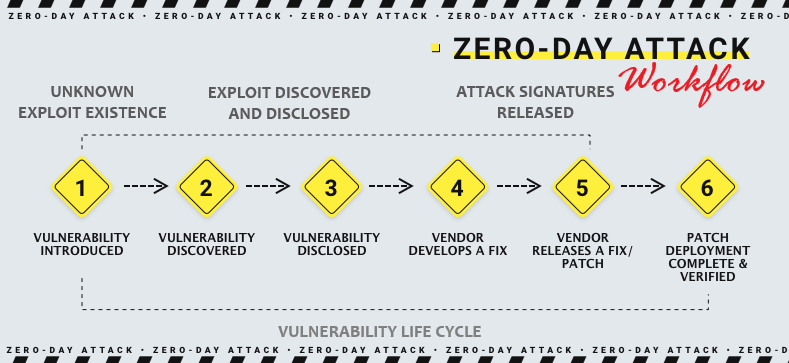
\includegraphics[width=1\linewidth]{image.png}
    \caption{Enter Caption}
    \label{fig:image-placeholder}
\end{figure}
    

\section{Context and Motivation}

% Always give a unique label
% and use \ref{<label>} for cross-references
% and \cite{<label>} for bibliographic references
% use \sectionmark{}
% to alter or adjust the section heading in the running head
In real-world enterprise AD environments, security teams - including systems administrators, incident responders, penetration testers, ethical hackers, and auditors - face a common challenge: ensuring the confidentiality, integrity, and availability of Active Directory in the face of growing complexity and increasingly advanced threat actors. AD is not only large, but also dynamic; users and permissions change constantly, and many of the risks lie in subtle or long-standing configurations rather than in overt malware or intrusions.

Defenders and security professionals must often sift through thousands of users, groups, and permissions, looking for signs of privilege abuse, security control tampering, inappropriate delegations, or dormant attack vectors, such as forgotten active user accounts that should have been disabled or deleted the moment the user was escorted off-premises. In many organizations, this work is often done manually, using a mix of graphical tools and ad hoc scripts. Unfortunately, this approach is not scalable and, sometimes, not feasible. It is slow, time-consuming, error-prone, and difficult to reproduce - particularly when trying to compare the state of AD over time for security baselining purposes or during an incident response investigation.

BTA was developed to bridge this gap. It automates deep inspection of AD data extracted from Domain Controllers, providing consistent outputs and facilitating offline analysis. Its goal is to simplify the process of identifying common AD abuses and to empower defenders to spot persistent misconfigurations before attackers do.

Among the key use cases addressed by BTA are:
    
\section{Understanding the Threat: Threat Hunting Backdoors}

To understand how attackers can abuse AD, we examine two realistic and commonly exploited backdoor mechanisms: manipulation of the Domain Admins group and the misuse of the AdminSDHolder
 object. These examples are not hypothetical - they are based on real-world abuse patterns observed during red team exercises and post-compromise investigations.

\section{Backdoor 1: Domain Admin Group Manipulation}

The Domain Admins group is one of the most powerful entities in an Active Directory domain. Its members effectively have full domain control over domain-wide resources. As such, it is a critical group that needs continuous monitoring, should be tightly and strictly administered and maintained and rarely changed. Yet attackers often target it directly or indirectly to establish initial access and persistence.

One popular technique involves obtaining the ability to \textbf{add or remove members} from the group. This does not always require being a Domain Admin initially. An attacker who compromises an account with GenericAll access to the Domain Admins group object can silently add another user, service account, or even a malicious script to the group without being noticed by traditional security tools and detection mechanisms.

In some instances, attackers don't just add users - they embed (and sometimes hard-code) permissions that allow them to re-add accounts later, even after an administrator believes they have removed the threat completely. These changes may be hidden within nested groups or disguised through indirect delegation.

These subtle forms of access manipulation are difficult to detect manually. The key challenge lies in identifying \textbf{who has effective control over the group} - not just who appears as a member. That requires a full audit of the group's security descriptor, including inherited and delegated permissions, and a recursive understanding of group nesting in Active Directory.
Please note that the first line of text that follows a heading is not indented, whereas the first lines of all subsequent paragraphs are.
